
Artificial neural networks (ANNs) are a machine learning approach to classification/regression problems, consisting of stacked layers of neurons implementing a nonlinear activation function interlinked with linear synapses. 
For our purposes, the activation function $g(x)$ is taken as a sigmoid and the output node a single logistic regression node, this class of ANNs are called Multilayer Perceptrons (MLPs). 

\begin{figure}[htbp]
	\centering
		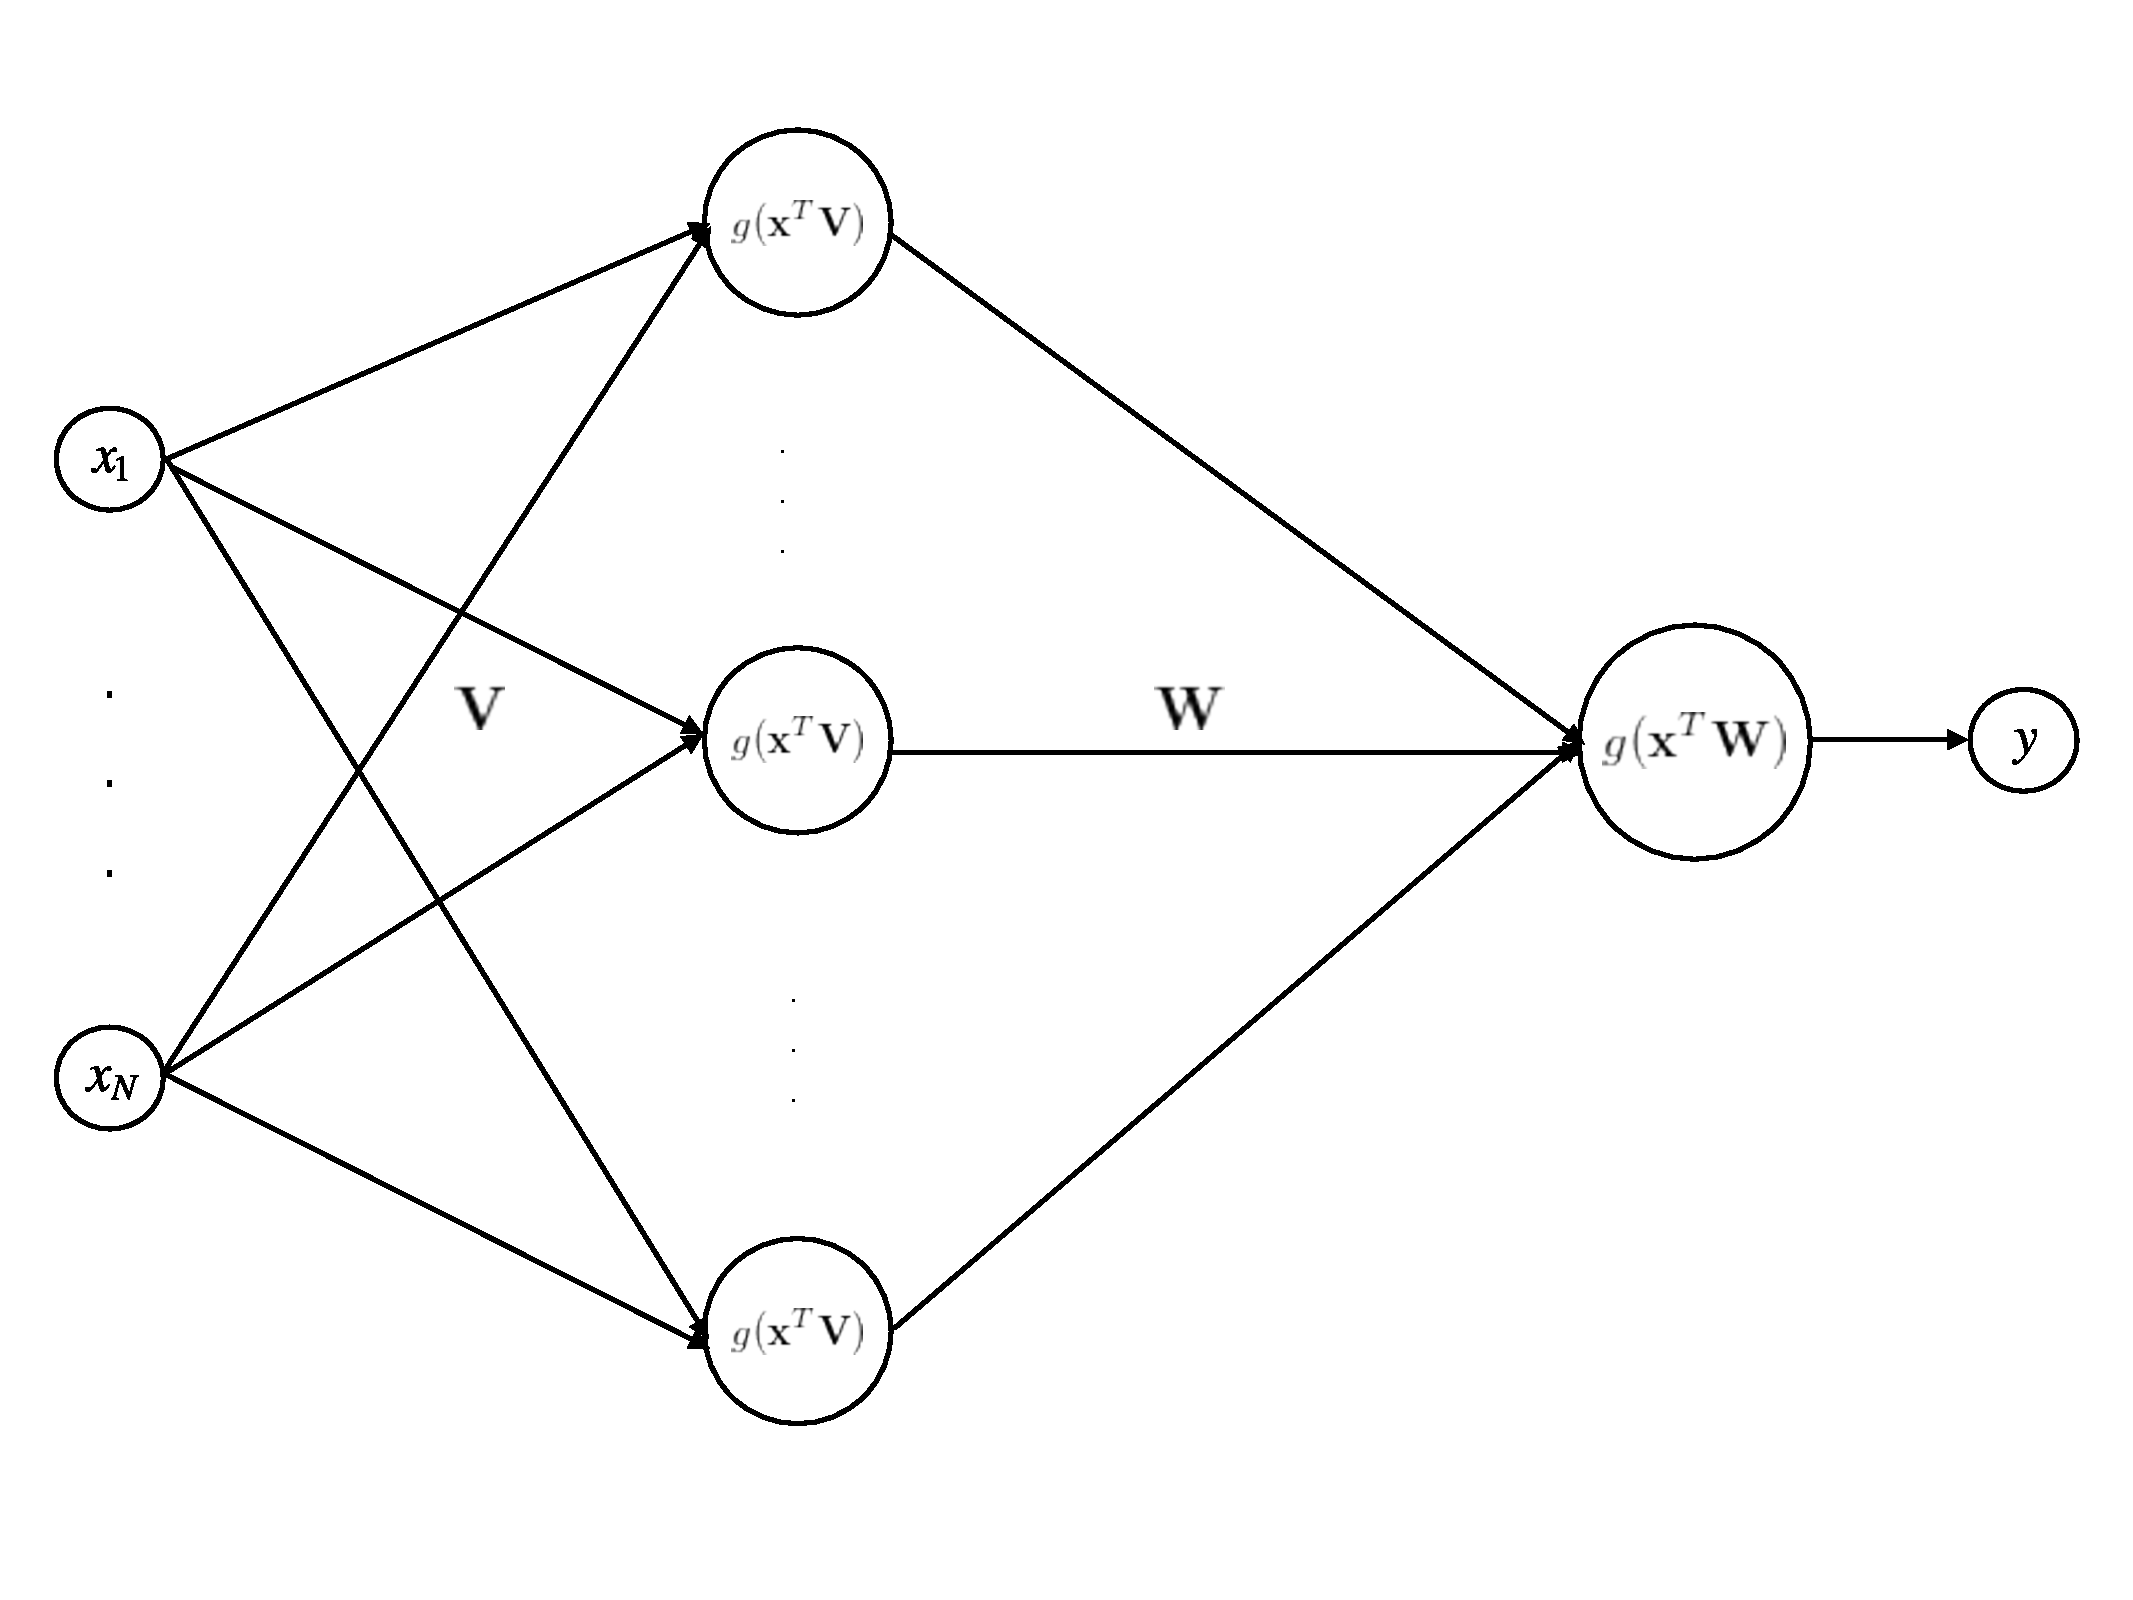
\includegraphics[width=0.7\linewidth]{img/ann_diag}
	\caption{An example MLP with one hidden layer, $N$ input variables $\mathbf{x}$ and single output $ 0 < y < 1$. The transfer function  $ g(\mathbf{x^T V}) = \frac{1}{1+e^{-\mathbf{x^TV}}}$  is sigmoid and the weight matrices are \textbf{V} and \textbf{W} }
	\label{ann_diag}
\end{figure}  

As a supervised machine learning problem, ANNs are trained by minimising the negative log likelihood (NLL) function $L(\mathbf{W})$ w.r.t. the parameters, 

\begin{align}
	L(\mathbf{W}) &= -\log\left[ P(\mathbf{W} | \mathcal{D}) \right] \\
				  &= -\sum_{i = 1}^{N_{train}} \left[ y^i\log \hat{y}^i + (1-y^i)\log(1-\hat{y}^i)\right]
\end{align}

where \textbf{W} denotes the weight matrices collectively and $\mathcal{D}$ the data.
Due to the nonlinearity of the activation function the NLL is a non-convex function of \textbf{W}, so it is minimised using random restarts of stochastic gradient descent. 
A strength of ANNs is that the gradient of the NLL can be efficiently computed by the backpropagation algorithm \cite{murphy2012machine}, which allows that gradient at the $n$th hidden layer to be calculated in terms of the error at the $(n+1)$th layer, so computation can start at the output layer and work backwards.
Once the gradient has been calculated the weights are optimised and the output estimates $\hat{y}$ updated by forward propagating the inputs through the network. A single backpropagation, optimisation, forward propagation cycle is called an epoch.
In order to avoid overfitting, the input data is split and 50\% reserved as a ``test set'' . 
After each epoch the network is evaluated on the on the test set and the misclassification error 
$e = \frac{1}{N_{test}}\sum_{i = 1}^{N_{test}} 1\{y^i \ne \hat{y}^i \} $
calculated, training is stopped when $e$ stops declining significantly.
We used the Cern ROOT \cite{citeulike:363715} implementation of an MLP, \texttt{TMultiLayerPerceptron} due to its tight integration with the rest of the ROOT data analysis frame, despite it lacking some desirable features.